% Chapter 17 homework
\documentclass[letterpaper,11pt]{article}
\usepackage[margin=0.5in]{geometry}
\usepackage{commath}
\usepackage{amsfonts}
\usepackage{amsmath}
\usepackage{graphicx}
\pagestyle{empty}
\begin{document}



% Heading
\begin{center}
	\bf
	ASTRONOMY 150: HOMEWORK 4 - SAM HEMANN
\end{center}



% 26
\paragraph{26.}
\it
An astronomer sees a redshift in the spectrum of an object. Without any other information, can she determine whether this is an extremely dense object (exhibiting gravitational redshift) or one that is receding from her (exhibiting Doppler redshift)? Explain your answer.
\smallskip
	\par
	\normalfont
	 With no other information, there is no way to distinguish gravitational redshift from Doppler redshift. Gravitational redshift is a result of relative time dilation slowing down the observed frequency of light - and thus longer wavelength since $v=f\lambda$. Doppler redshift is the wavelength of emitted light being ``stretched'' as an object moves further away, so the observed effects of each phenomenon are identical.



% 29
\paragraph{29.}
\it
Twin A takes a long trip in a spacecraft and returns younger than twin B, who stayed behind. Could twin A ever return before twin B was born? Explain.
\smallskip
	\par
	\normalfont
	Well this chapter didn't cover wormholes, so assuming this question is only referencing time dilation then no, twin A could not return before twin B was born. An object can approach effectively being ``frozen'' in time as it's velocity approaches the speed of light (relative to an observer), but time will never move backwards due to dilation.



% 34
\paragraph{34.}
\it
Looking into a speeding spaceship, you observe that the travelers are playing soccer with a perfectly round soccer ball. What is the shape of the ball according to observers on the spacecraft? **Add: Draw two sketches of the spacecraft and ball as perceived by: (1) you as the external observer, and (2) the spacecraft travelers. Note the direction of travel in your sketch, and clearly depict the shape of the ball for each reference frame sketch.
\smallskip
	\par
	\normalfont
	Since objects appear shorter as they move faster, the ball would appear as an elongated sphere to observers on the spacecraft - like a football with less pointy ends.
	\begin{figure}[h]
		\centering
		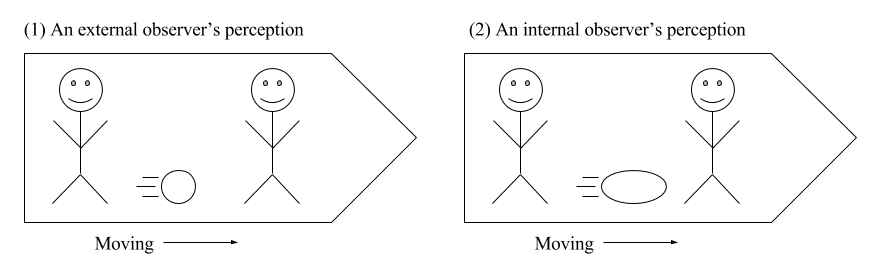
\includegraphics[scale=0.5]{hw4sketch}
	\end{figure}



% 36
\paragraph{36.}
\it
Of the four forces in nature (strong nuclear, electromagnetic, weak nuclear, and gravity), gravity is by far the weakest. Why, then, is gravity such a dominant force in stellar evolution? (Note: The weak nuclear force, which has not been discussed in this text yet, is involved in certain decay processes within the nucleus.)
\smallskip
	\par
	\normalfont
	Gravity has essentially infinite range, and unlike electromagnetism it always attracts and never repels. Also, since it interacts with anything that has a mass, it's great at bringing matter together, which is basically the core principle of star formation and evolution.



% 37
\paragraph{37.}
\it
Suppose astronomers discover a 3-$M_\oplus$ black hole located a few light-years from Earth. Should they be concerned that its tremendous gravitational pull will lead to Earth’s untimely demise?
\smallskip
	\par
	\normalfont
	No. Black holes do not ``suck'' up material around them, so it's effect on Earth would be no different than a 3-$M_\oplus$ star nearby. Also ``a few light-years'' is such a large distance that even if the solar system and black hole were on a collision course we'd have plenty of time to come up with a solution.
\bigskip

\begin{center}
	\it
	(Continued on back)
\end{center}
\pagebreak

% 52
\paragraph{52.}
\it
The Moon has a mass equal to $3.7 \times 10^{-8}M_\oplus$. Suppose the Moon suddenly collapsed into a black hole.
\smallskip
\par
\it
a. What would be the radius of the event horizon (the “point of no return”) around the black-hole Moon?
\smallskip
	\par
	\normalfont
	\begin{center}
	$
	\displaystyle
	r
	=
	\frac{2GM_{\textrm{BH}}}{c^2}
	=
	3 \textrm{ km} \times \frac{M_\textrm{BH}}{M_{\oplus}} \textrm{[pg.570]}
	=
	(3 \textrm{ km})( 3.7 \times 10^{-8}M_\oplus)
	=
	1.11 \times 10^{-7} \textrm{ km}
	=
	0.111 \textrm{ mm}
	$
	\end{center}
	\bigskip

\par
\it
b. What effect would this collapse have on tides raised by the Moon on Earth? Explain.
\smallskip
	\par
	\normalfont
	The tides wouldn't change at all, since they are caused by the gravitational of the Moon's mass, not its size.
	\bigskip

\par
\it
c. Do you think this event would generate gravitational waves? Explain.
\smallskip
	\par
	\normalfont
	Probably not, since there is such a small mass collapsing in a uniform manner. It takes a very large mass moving incredibly fast for waves to be generated.


\end{document}
